\section{Auswertung}

\subsection{Apparatekonstanten}

\begin{itemize}
  \item Masse der Billardkugel: $m_K = \SI{142,1(0)}{\g}$
  \item Radius der Billardkugel: $r_K = \SI{2,55(0)}{\cm}$
  \item Trägheitsmoment: $J_K = \SI{3,696(0)e-5}{\kg\m^2}$
  \item verschiebbare Masse: $m = \SI{1,4(0)}{\g}$
  \item Erdbeschleunigung: $g = \SI{10(0)}{\meter \per \square \second}$
\end{itemize}

\subsection{Gravitation}

Das magnetische Feld, das gegen den Radius aufgetragen werden soll, ergibt sich aus Gleichung \eqref{eqn:bfeld}.
\begin{table}
  \centering
  \caption{Messdaten \enquote{Gravitation}}
  \label{tab:grav}
  \begin{tabular}{S S S}
    \toprule
      {$r \:/\: \mathrm{cm}$} & {$I \:/\: \mathrm{A}$} & {$B \:/\: \mathrm{mT}$}\\
    \midrule
    1,8	 & 	1,5 	& 	2,03 \\
    3,3	 & 	1,9 	& 	2,58 \\
    3,8	 & 	2,0 	& 	2,71 \\
    4,3	 & 	2,1 	& 	2,85 \\
    4,8	 & 	2,2 	& 	2,98 \\
    5,5	 & 	2,4 	& 	3,25 \\
    6,0	 & 	2,5 	& 	3,39 \\
    6,7	 & 	2,7 	& 	3,66 \\
    7,3	 & 	2,8 	& 	3,80 \\
    7,5	 & 	3,0 	& 	4,07 \\
    \bottomrule
  \end{tabular}
\end{table}
\newpage
Aus diesen Messwerten folgt der Graph:
\begin{figure}[H]
  \centering
  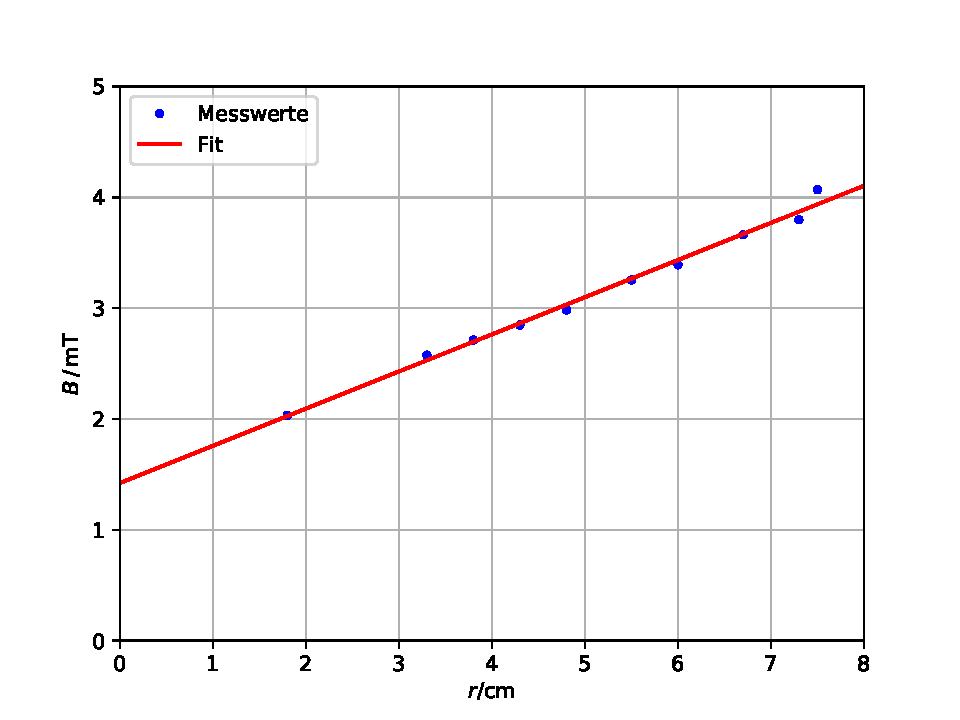
\includegraphics[width=\textwidth]{Plots/grav.pdf}
  \caption{$r$-$B$-Diagramm zur Bestimmung des magnetischen Moments}
  \label{fig:grav}
\end{figure}
Zur Bestimmung des magnetischen Moments wird eine lineare Regression durchgeführt, die folgende Werte liefert:
\begin{table}[H]
  \centering
  \caption{lineare Regression}
  \label{tab:lin1}
  \begin{tabular}{l c}
    \toprule
       & {Werte}\\
    \midrule
    Steigung m & \SI{0,0335(11)}{\tesla \per \meter} \\
    Achsenabschnitt b & \SI{0,0014(0)}{\tesla} \\
    \bottomrule
  \end{tabular}
\end{table}
Das magnetische Moment ergibt sich aus der in Gleichung \eqref{eqn:mygrav} gegebenen Steigung:
$\mu_{\symup{Dipol}} = \SI{0,4179(173)}{\ampere \square \meter}$.
%\newpage

\subsection{Schwingungsdauer}
Wie schon im vorausgegangenen Kapitel berechnet sich auch hier, die benötigte magnetische Feldstärke
aus Gleichung \eqref{eqn:bfeld}.
Alle benötigten Messdaten finden sich in nachfolgender Tabelle:
\begin{table}[H]
  \centering
  \caption{Messdaten \enquote{Schwingungsdauer}}
  \label{tab:schw}
  \begin{tabular}{S S S S S}
    \toprule
      {$I \:/\: \mathrm{A}$} & {$T_{10} \:/\: \mathrm{s}$} &
      {$T \:/\: \mathrm{s}$} & {$B^{-1} \:/\: \mathrm{T^{-1}}$} & {$T^2 \:/\: \mathrm{s^2}$}\\
    \midrule
    0,5  &	24,85  & 	2,49	&	 1474,83 &  6,18 \\
    1,0  &	15,33  & 	1,53	&	 737,41	 &	2,35 \\
    1,5  &	14,09  & 	1,41	&	 491,61	 &	1,99 \\
    2,0  &	11,97  & 	1,20	&	 368,71	 &	1,43 \\
    2,2  &	10,67  & 	1,07	&	 335,19	 &	1,14 \\
    2,5  &	9,93	 &  0,99	&	 294,97	 &	0,99 \\
    3,0  &	9,20	 &  0,92	&	 245,80	 &	0,85 \\
    3,5  &	8,85	 &  0,89	&	 210,69	 &	0,78 \\
    3,8  &	11,35  & 	1,14	&	 194,06	 &	1,29 \\
    4,0  &	8,99	 &  0,90	&	 184,35	 &	0,81 \\
    \bottomrule
  \end{tabular}
\end{table}
Daraus folgt der Graph:
\begin{figure}[H]
  \centering
  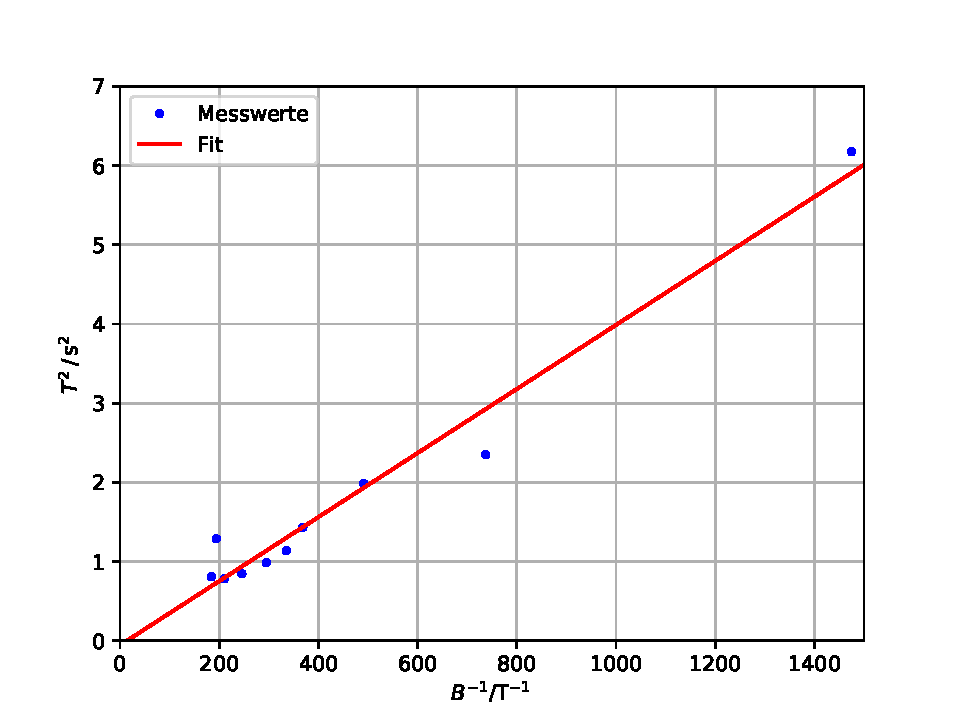
\includegraphics[width=\textwidth]{Plots/schw.pdf}
  \caption{$B^{-1}$-$T^2$-Diagramm zur Bestimmung des magnetischen Moments}
  \label{fig:schw}
\end{figure}

\begin{table}[H]
  \centering
  \caption{lineare Regression}
  \label{tab:lin2}
  \begin{tabular}{l c}
    \toprule
       & {Werte}\\
    \midrule
    Steigung m & \SI{0.0040(3)}{\square \second \tesla} \\
    Achsenabschnitt b & \SI{-0.0554(1558)}{\square \second} \\
    \bottomrule
  \end{tabular}
\end{table}
Aus Gleichung \eqref{eqn:sdauer} berechnet sich das magnetische Moment
$\mu_{\symup{Dipol}} = \SI{0,3609(236)}{\ampere \square \meter}$.
%\newpage
\subsection{Präzession}

Zur Aufnahme der Messreihe wurde das Stroboskop auf die Frequenz $\nu = 5 \si{Hz}$ eingestellt.
\begin{table}[H]
  \centering
  \caption{Messdaten \enquote{Präzession}}
  \label{tab:prae}
  \begin{tabular}{S S S S S S c S c}
    \toprule
      {$I \:/\: \mathrm{A}$} & & \multicolumn{3}{c}{$T_P \:/\: \mathrm{s}$} & &
      {$T_{\diameter}  \:/\: \mathrm{s}$} & {$B \:/\: \mathrm{mT}$} &
      {$T_{\diameter}^{-1} \:/\: \mathrm{mHz}$}\\
    \midrule
    0,5  & &	22,58  &	21,26	 &  18,12	 & &  20,65	\pm 1,32	&	 0,68	 &  48,42  \pm 3,10 \\
    1,0  & &	11,64  &	12,39	 &  11,30	 & &  11,78	\pm	0,32  &	 1,36	 &  84,91  \pm 2,32 \\
    1,5  & &	8,07	 &  7,64	 &  7,31	 & &  7,67	\pm 0,22	&  2,03	 &	130,32 \pm 3,74 \\
    2,0  & &	6,01	 &  6,22	 &  6,00	 & &  6,08	\pm 0,07	&  2,71	 &	164,56 \pm 1,94 \\
    2,2  & &	5,90	 &  5,64	 &  5,77	 & &  5,77	\pm 0,08	&  2,98	 &	173,31 \pm 2,25 \\
    2,5  & &	4,75	 &  4,53	 &  4,76	 & &  4,68	\pm 0,08	&  3,39	 &	213,68 \pm 3,43 \\
    3,0  & &	4,33	 &  4,35	 &  4,18	 & &  4,29	\pm	0,05  &  4,07	 &	233,28 \pm 2,92 \\
    3,5  & &	3,29	 &  3,41	 &  3,27	 & &  3,32	\pm 0,04	&  4,75	 &	300,90 \pm 3,96 \\
    3,8  & &	3,39	 &  3,42	 &  3,45	 & &  3,42	\pm	0,02  &  5,15	 &	292,40 \pm 1,48 \\
    4,0  & &	3,17	 &  3,20	 &  3,17	 & &  3,18	\pm	0,01  &  5,42	 &	314,47 \pm 0,99 \\
    \bottomrule
  \end{tabular}
\end{table}
Die Fehler von $T_{\diameter}$, die der Formel
\begin{equation}
  \delta = \sqrt{\frac{1}{n^2-n} \cdot \sum_{i=1}^{n}(x_i - \bar {x})^2}
\end{equation}
entstammen, ergeben in Kombination mit der Gauß'schen Fehlerfortpflanzung
\begin{equation}
  \delta = \sqrt{ \sum_{i=1}^{n}(\frac{\partial y}{\partial x_i} \Delta x_i)^2}
\end{equation}
die Fehler von $\frac {1}{T_{\diameter}}$.
\newpage
Der dazugehörige Graph ist:
\begin{figure}[H]
  \centering
  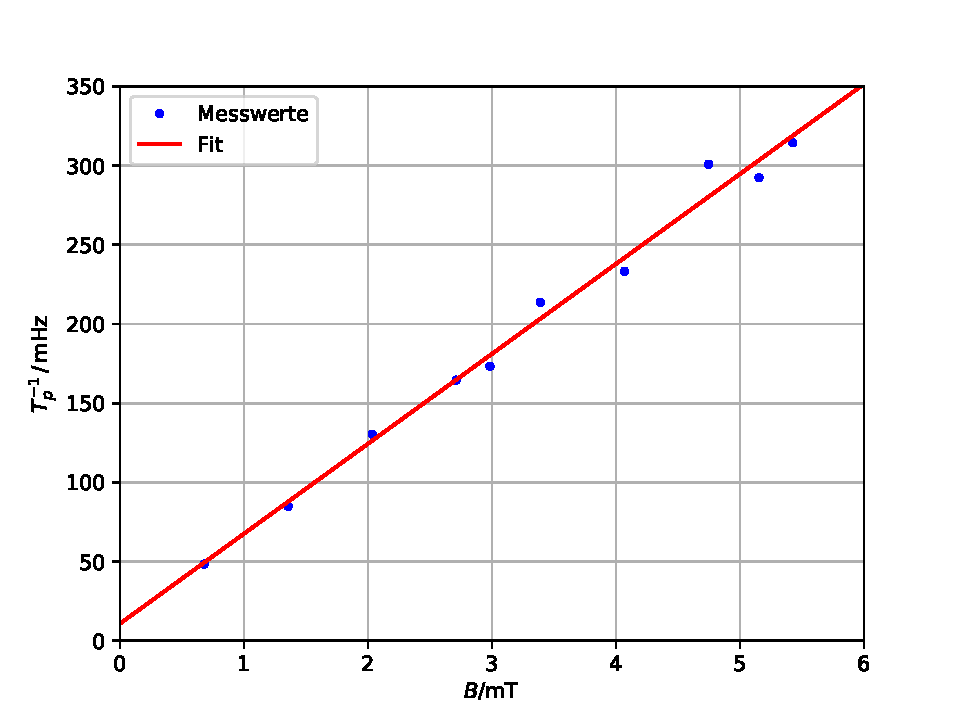
\includegraphics[width=\textwidth]{Plots/prae.pdf}
  \caption{$B$-$T_P^{-1}$-Diagramm zur Bestimmung des magnetischen Moments}
  \label{fig:prae}
\end{figure}
Hier ergibt sich aus der linearen Regression:
\begin{table}[H]
  \centering
  \caption{lineare Regression}
  \label{tab:lin3}
  \begin{tabular}{l c}
    \toprule
       & {Werte}\\
    \midrule
    Steigung m & \SI{56.7703(20932)}{\hertz \per \tesla} \\
    Achsenabschnitt b & \SI{0.0109(75)}{\hertz} \\
    \bottomrule
  \end{tabular}
\end{table}
Aus Gleichung \eqref{eqn:pfrq} ergibt sich $\mu_{\symup{Dipol}} = \SI{0.4141(153)}{\ampere \square \meter}$.
